\chapter{Network Security}
Netzwerkangriffe können auf unterschiedliche Arten, unterschiedlichen Ebenen und verschiedene Protokolle stattfinden. Deshalb muss bei einem Security-Konzept möglichst alles berücksichtigt werden.
\begin{table}[H]
	\begin{tabular}{|l|l|l|}
		\hline
		\multicolumn{1}{|c|}{\textbf{Angriffe}} & \multicolumn{1}{c|}{\textbf{OSI-Modell}} & \multicolumn{1}{c|}{\textbf{Abwehr}} \\ \hline
		\begin{tabular}[c]{@{}l@{}}Social Engineering\\ Passwörter\\ Pretexting\end{tabular} & L8-Mensch & \begin{tabular}[c]{@{}l@{}}Schulungen\\ Vernünftig und vorsichtiges \\ handeln\end{tabular} \\ \hline
		\begin{tabular}[c]{@{}l@{}}SQL-Injection\\ Wurm, Virus, Trojaner\\ Ransomware, Spyware\\ Protokolle (HTTP, FTP, \\ Telnet, DHCP, DNS,...)\end{tabular} & \begin{tabular}[c]{@{}l@{}}L7-Application\\ L6-Presentation\\ L5-Session\end{tabular} & \begin{tabular}[c]{@{}l@{}}Firewall, IPS, IDS, ESA, WSA\\ Eingabeüberorpfung\\ gute Software \& Protokolle\\ End-Point-Detection\\ Anti-Virus, Updates\end{tabular} \\ \hline
		\begin{tabular}[c]{@{}l@{}}DDOS\\ $\rightarrow$ TCP (SYN-Flood,\\ $\rightarrow$ UDP\end{tabular} & L4-Transport & \begin{tabular}[c]{@{}l@{}}IPS, IDS\\ Firewall, ACL\end{tabular} \\ \hline
		\begin{tabular}[c]{@{}l@{}}Routing, DDoS\\ MITM, IP-Spoofing\\ Protokolle (ICMP,\end{tabular} & L3-Network & \begin{tabular}[c]{@{}l@{}}Firewall, ACL, IPS, IDS\\ sichere Protokolle (IPsec)\end{tabular} \\ \hline
		\begin{tabular}[c]{@{}l@{}}MITM: ARP-Spoofing, MAC-Spoofing\\ DDOS: MAC-Flooding\\ Protokolle (STP, CDP)\end{tabular} & L2-Data Link & \begin{tabular}[c]{@{}l@{}}MAC-Filter, AAA\\ sichere Protokolle\\ Verschlüsselung\end{tabular} \\ \hline
		\begin{tabular}[c]{@{}l@{}}DoS (Störsender, Zerstörung \\ der Infrastruktur)\\ Physischer Zugang\\ MITM, Hardware\end{tabular} & L1-Physical & \begin{tabular}[c]{@{}l@{}}Zutrittskontrolle\\ Backups\end{tabular} \\ \hline
	\end{tabular}
\end{table}
Dem Angreifer reicht eventuell ein einziger Angriffspunkt im Netz. Meist sind die User (Personen) das größte Problem. $\rightarrow$ \textbf{''Der Angreifer muss nur einmal gewinnen''}

\subsection*{Sicherheitsrichtlinien}
\begin{tabular}{ | p{\dimexpr 0.5\linewidth-2\tabcolsep} | p{\dimexpr 0.5\linewidth-2\tabcolsep} |} \hline
	\textbf{User} & \textbf{Unternehmen} \\ \hline
	$\bullet$ Passwörter (Mindestlänge, eins pro Account, keine persönlichen Daten) & $\bullet$ Passwortrichtlinien, User Verwaltung, Recht vergeben \\
	$\rightarrow$ Passwortmanager, 2FA & $\bullet$ Firmengeräte, spezielle Rechte, wie beim User \\
	$\bullet$ Datenverwaltung (Wann?, Wo?, Welche?, Wann?,...) & $\bullet$ DMZ, VPN, Firewall, IPS, IDS, WSA, ESA \\
	$\bullet$ Firewall & $\bullet$ Zugangskontrollen \\
	$\bullet$ Updates (OS, Software) & $\bullet$ Schulung der Mitarbeiter \\
	$\bullet$ Antivirus/Antispysoftware & $\bullet$ Backups \\
	$\bullet$ Vernünftig handeln & $\bullet$ Pen-Testing \\
	 & $\bullet$ Risikoanalyse $\rightarrow$ Schwachstellen kennen \\
	 & $\bullet$ Verhaltensanalyse \\
	 & $\bullet$ Datatransfer sichtbar machen \\
	\hline
\end{tabular} 

\section{Firewall}
Mit einer Firewall kann der eingehende/ausgehende Datenverkehr kontrolliert, protokolliert und gefiltert werden (sperren, freigeben).

\subsection*{Unterscheidung nach Position}
\begin{itemize}
	\item \textbf{Personal Firewall} (am eigenen Gerät) z.B. Windows Defender, UFW,...
	\item \textbf{External Firewall} (zwischen lokalen \& globalen Netz) z.B. ASA, Fortinet, Barracuda, PFSense,...
\end{itemize}

\subsection*{Unterscheidung nach Funktion}
\begin{itemize}
	\item (L4) \textbf{Paketfilter:} IP-Adressen, Ports z.B. ACL
	\item (L4) \textbf{Stateful Inspection:} Untersucht die ganze Sitzung (mehrere Aufrufe zu z.B. gleiche IPs)
	\item (L7) \textbf{Application Firewall:} Proxy Server
	\item (Daten) \textbf{Deep Paket Inspection Firewall}
\end{itemize}

Eine falsch konfigurierte Firewall bietet keinen Schutz. Eine Firewall muss ständig gewartet und aktualisiert werden.

\section{IDS \& IPS}
\begin{figure}[H]
	\centering
	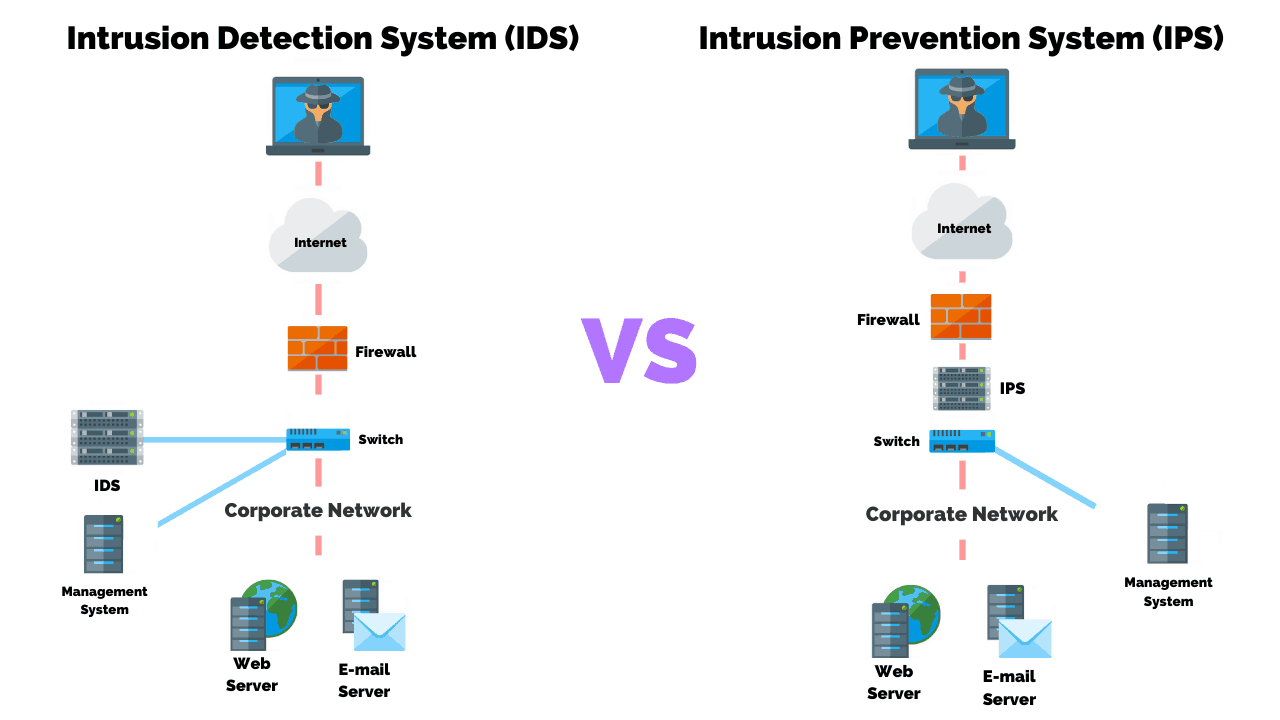
\includegraphics[width=0.8\linewidth]{figures/ids_ips.png}
	\caption{IPS \& IDS}
\end{figure}

\begin{tabular}{ | p{\dimexpr 0.5\linewidth-2\tabcolsep} | p{\dimexpr 0.5\linewidth-2\tabcolsep} |} \hline
	\textbf{IDS (Intrusion Detection System)} & \textbf{IPS (Intrusion Prevention System)} \\ \hline
	Wird nur parallel informiert & Alles muss über IPS \\
	+ schneller (da es parallel ist) & - langsamer (da seriell) \\
	- nur Warnungen & + sicherer \\
	\hline
\end{tabular} 

\section{Honeypot}
\begin{figure}[H]
	\centering
	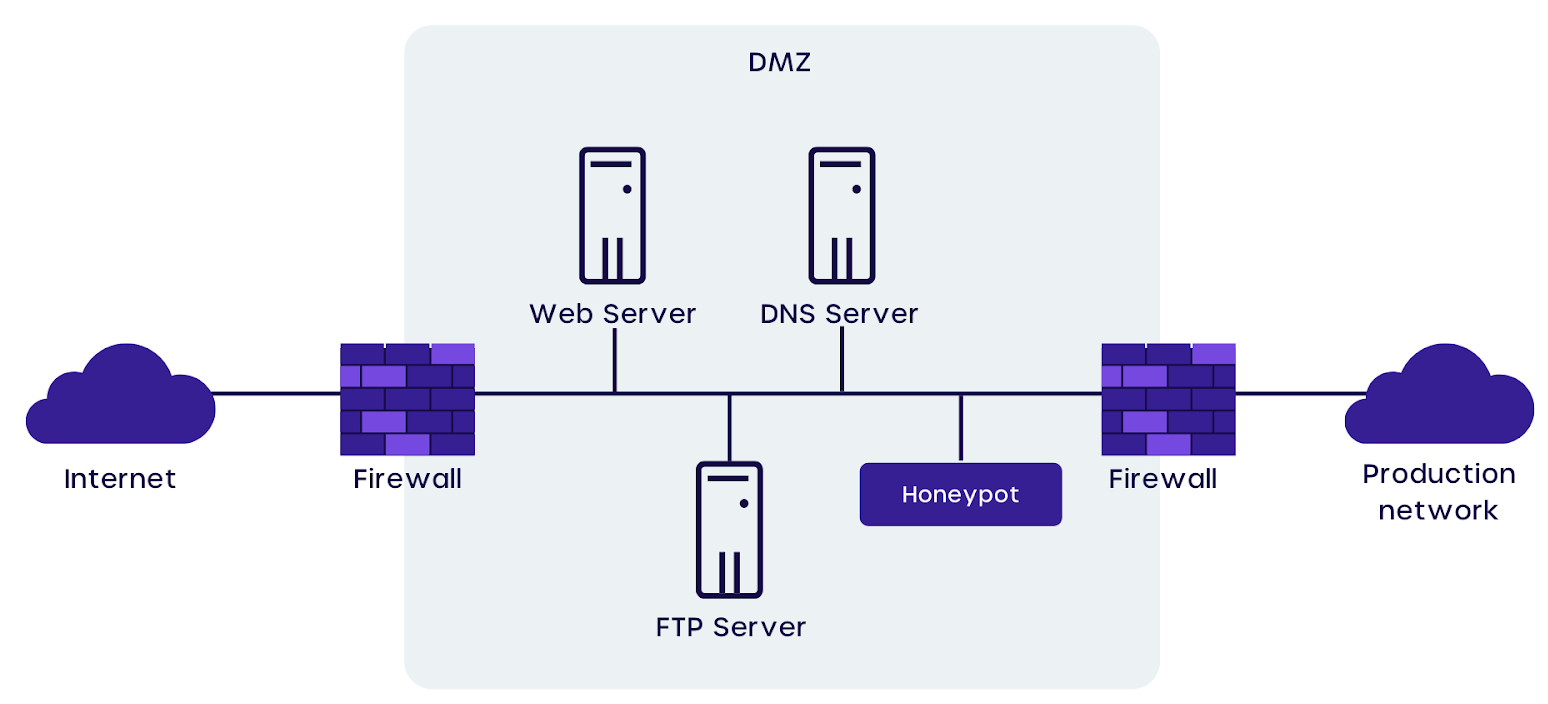
\includegraphics[width=0.8\linewidth]{figures/honeypot.png}
	\caption{Honeypot}
\end{figure}
Bei einem Honeyport werden bewusst veraltete Software \& Hardware für Angreifer als Köder aufgestellt. 

\section{VPN} 
Erstellt eine verschlüsselte Verbindung zu einem entfernten VPN-Server.

\begin{figure}[H]
	\centering
	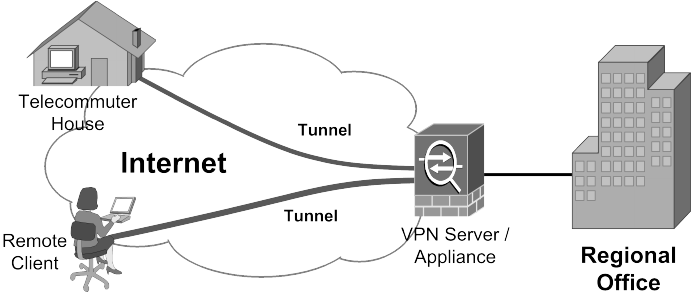
\includegraphics[width=0.8\linewidth]{figures/vpn.png}
	\caption{VPN}
\end{figure}
\subsection*{Arten von VPN}
\begin{itemize}
	\item Ende-zu-Ende VPN
	\item Ende-zu-Netz VPN
	\item Netz-zu-Netz VPN
\end{itemize}

\section{ESA (Email Security Appliance) \& WSA (Web Security Appliance)}
Funktioniert wie ein Proxy-Server, spezifisch für Email/Web.
\begin{figure}[H]
	\centering
	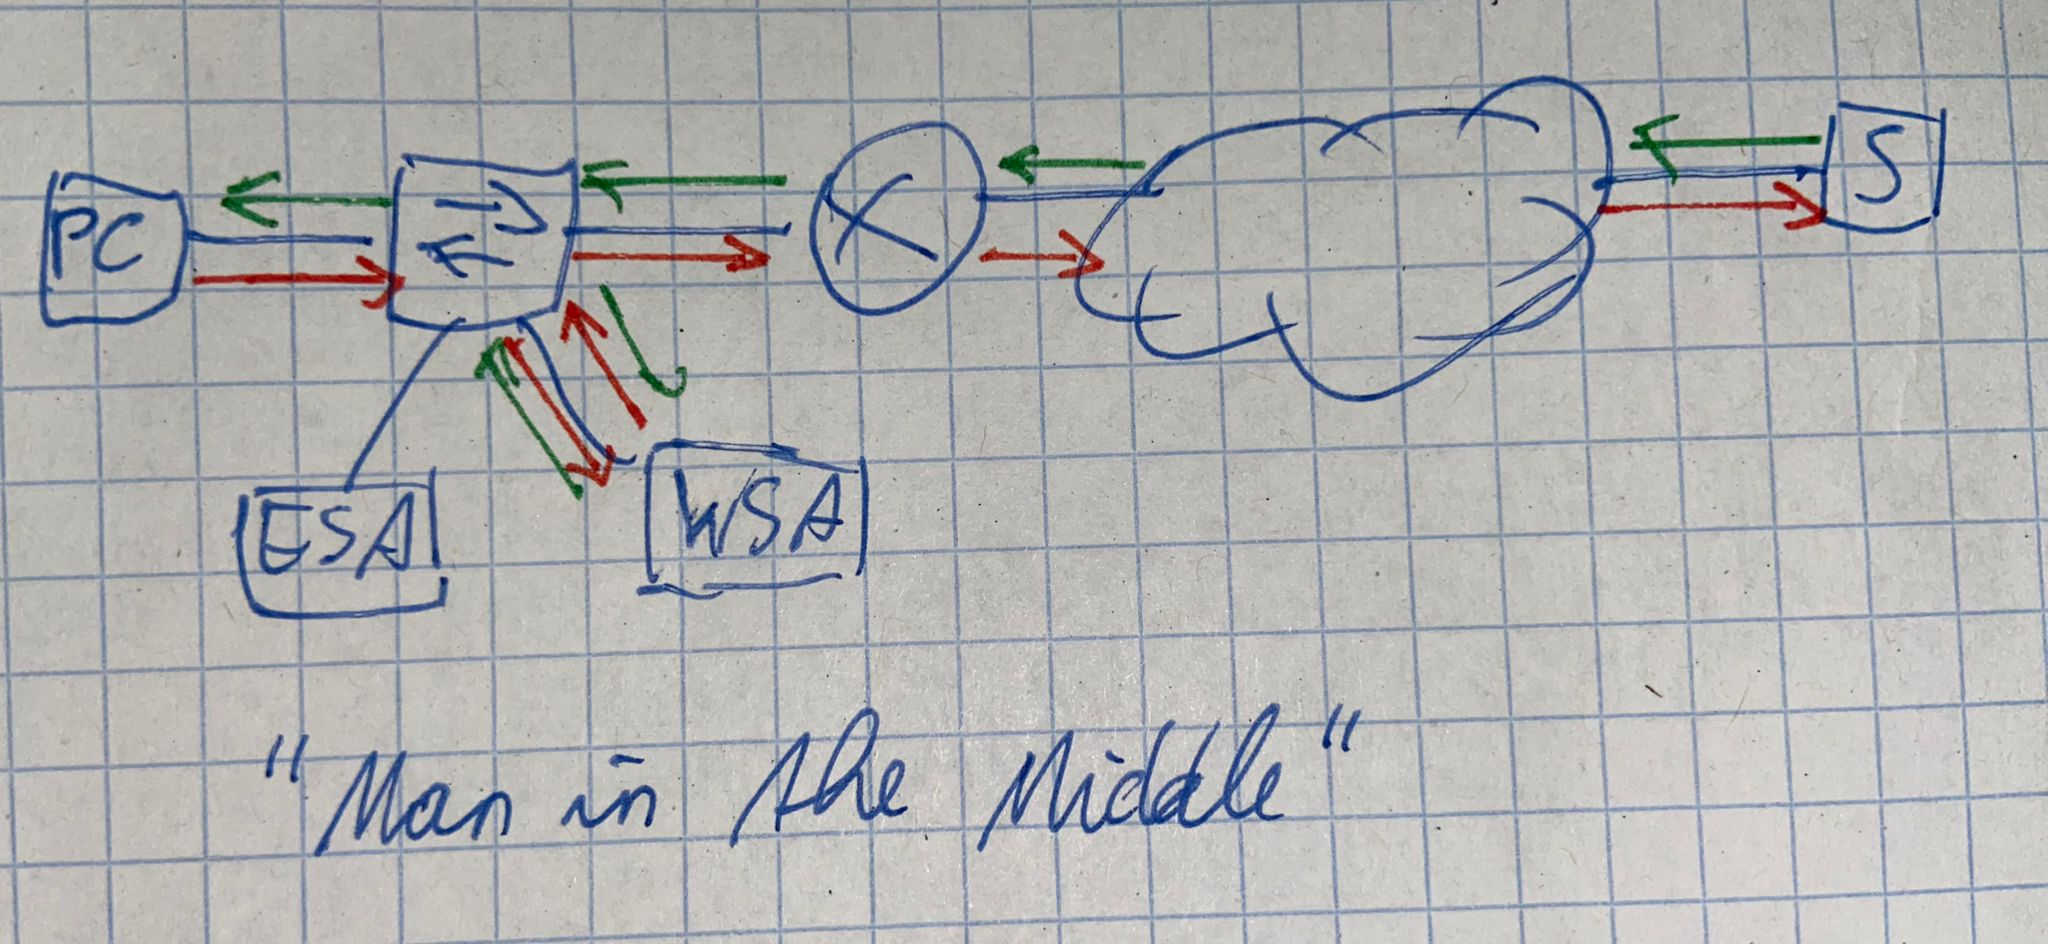
\includegraphics[width=0.8\linewidth]{figures/esawsa.jpeg}
	\caption{ESA \& WSA}
\end{figure}

\section{IPsec}
Ziel: Sicheres Protokoll zur Datenübertragung
\begin{itemize}
	\item \textbf{Transport-Modus:} Verschlüsselung ab L4 und fügt eine Authentifizierung in den Header ein.
	\item \textbf{Tunnel-Modus:} Alles wird verschlüsselt und es wird ein neuer verschlüsselter Header angehängt. Darin stehen die wichtigsten Felder (MAC, IP,...) + Authentifizierung
\end{itemize}